\section{Definició de conceptes}
\subsubsection{Anàlisi d'un tiquet}
Un tiquet d'incidències és un informe de qualsevol problema o dubte que hagi pogut sorgir, normalment, dins d'una empresa. Aquests tiquets serveixen per comunicar del problema mencionat al tiquet i s'espera obtenir una contestació detallant quins són els passos a seguir per solucionar el problema o una resposta resolent el dubte. Per aquest projecte, s'ha usat \textit{OTRS}, una eina de gestió i emmagatzematge de tiquets. Gràcies a la reducció de l'abast mencionat a l'apartat \ref{sec:gestio_risc}, només es poden trobar tiquets pertenyents a dues categories: \textit{phishing} i \textit{malware}, sent la primera més abundant. A continuació, es mostra un tiquet d'exemple d'ORTS i s'explica en deteniment les seves parts.
%(usuaris afectats, accions mitigació, accions control, url mail incident, from mail incident, recipient mail incident, subject mail incident)

En el tiquet es poden veure els següents camps:
\begin{enumerate}
    \item \textbf{Logo Znuny:} Tot i que a l'\textbf{Agència} s'utilitza \textit{OTRS}, aquest tiquet d'exemple, i les proves que s'han dut a terme han sigut realitzades amb Znuny. Znuny és la continuació d'\textit{OTRS}, ja que a partir en un cert punt, la versió gratuita d'\textit{OTRS} (\textit{OTRS Community Edition}) va deixar de rebre actualitzacions de manteniment. A efectes pràctics, Znuny és es comporta de manera idèntica i és compatible amb les mateixes llibreries que \textit{OTRS}. S'ha utilitzat per a totes les proves locals que requereixin el servei d'un gestor de tiquets.
    \item \textbf{Número del tiquet:} Número identificador únic del tiquet. És l'identificador principal per obtenir el tiquet de la base de dades.
    \item \textbf{Capçalera:} Els tiquets tenen un assumpte, remitent, destinatari i informació sobre la data d'enviament, igual que un correu electrònic. En aquest cas, està dividida en diversos llocs del tiquet.
    \item \textbf{Informació del tiquet (metadata):} Hi ha informació inclosa en el tiquet que permet establir alguns camps rellevants relatius a les condicions actuals del tiquet, tals com: l'estat del tiquet, la seva prioritat, a quina cua pertany, quant de temps fa que s'ha creat, etc.
    \item \textbf{Informació del client:} Conté informació sobre l'empresa que ha patit l'incident, així com l'usuari de l'empresa que ha escrit el tiquet.
    \item \textbf{Número de l'article:} Un tiquet es divideix en diferents articles. Cada article representa un missatge o correu que una de les parts ha enviat. En aquest exemple hi ha dos articles: El primer (\ref{fig:tiquet-exemple-2}) informant del problema i el segon (\ref{fig:tiquet-exemple-1}) explicant les mesures preses a causa de l'incident. És important tenir en compte que, tal com es veu a la Figura \ref{fig:tiquet-exemple-1}, el text de tots els anteriors tiquets es reescriu sota d'aquest.
\end{enumerate}

Tal i com s'ha explicat, la feina d'extracció dels camps succeeix majoritariament dins del tiquet, analitzant i extraient informació dels diferents articles. Aquests són els camps que es busquen, el seu identificador otorgat per l'\textbf{Agència} i la seva definició: 
\begin{enumerate}
  \setcounter{enumi}{6}
  \item \textbf{Usuaris afectats (\textit{usuarios\_afectados}):} Els usuaris afectats són tots aquells usuaris que han rebut el correu referent a la incidència. Aquests usuaris han de ser molt específics, es requereix que sigui els emails que han rebut aquest correu. No és correcte, per exemple, identificar pel seu nom als usuaris afectats, ni incloure tot un grup, com un departament sencer.
  \item \textbf{Accions de mitigació (\textit{acciones\_mitigacio}):} Les accions de mitigació són les accions preses per evitar l'expansió de l'incident. Normalment, les accions de mitigació són preses per l'equip de ciberseguretat encarregat de solucionar el tiquet, però pot arribar pels dos llocs. Són mesures immediates que només afecten la incidència concreta que s'intenta combatre, i aquest és el punt que més les diferencia de les accions de control.
  \item \textbf{Accions de control (\textit{acciones\_control}):} Les accions de control, a diferència de les accions de mitigació, són aquelles que s'utilitzen per prevenir més incidents del mateix estil. Són aquelles mesures que, estudiant el cas actual, es poden implementar i evitar així un rang més ampli d'aquests esdeveniments.
  \item \textbf{URL de l'incident (\textit{URL\_mail\_incident}):} És l'adreça electrònica que s'ha usat en el correu de l'incident per enganyar a la víctima i fer creure que estan en una pàgina web coneguda. Es fa ús d'una còpia exacta de la pàgina web per evitar sospites i així robar la informació de la víctima.
  \item \textbf{Mail de l'atacant (\textit{from\_mail\_incident}):} És l'adreça electrònica des de la qual es van enviar els correus maliciosos. Normalment, pertanyen a un domini estranger, o a un domini de correus temporals per evitar ser rastrejats. El nom d'usuari, però, és esperable que sigui un que simula ser una entitat real, per intentar enganyar a les víctimes.
  \item \textbf{Mail de la víctima (\textit{recipient\_mail\_incident}):} És un dels usuaris que ha rebut el correu maliciós (\textit{affected\_users}) ha sigut el primer a reportar o a informar sobre aquest succés.
  \item \textbf{Assumpte correu de l'incident (\textit{subject\_mail\_incident}):} És l'assumpte que tenia el correu de l'atacant. Solen ser assumptes molt cridaners amb paraules que inciten a actuar ràpidament, per aconseguir que la víctima entri sense pensar-s'ho dues vegades.
\end{enumerate}

\begin{figure}[H]
    \centering
    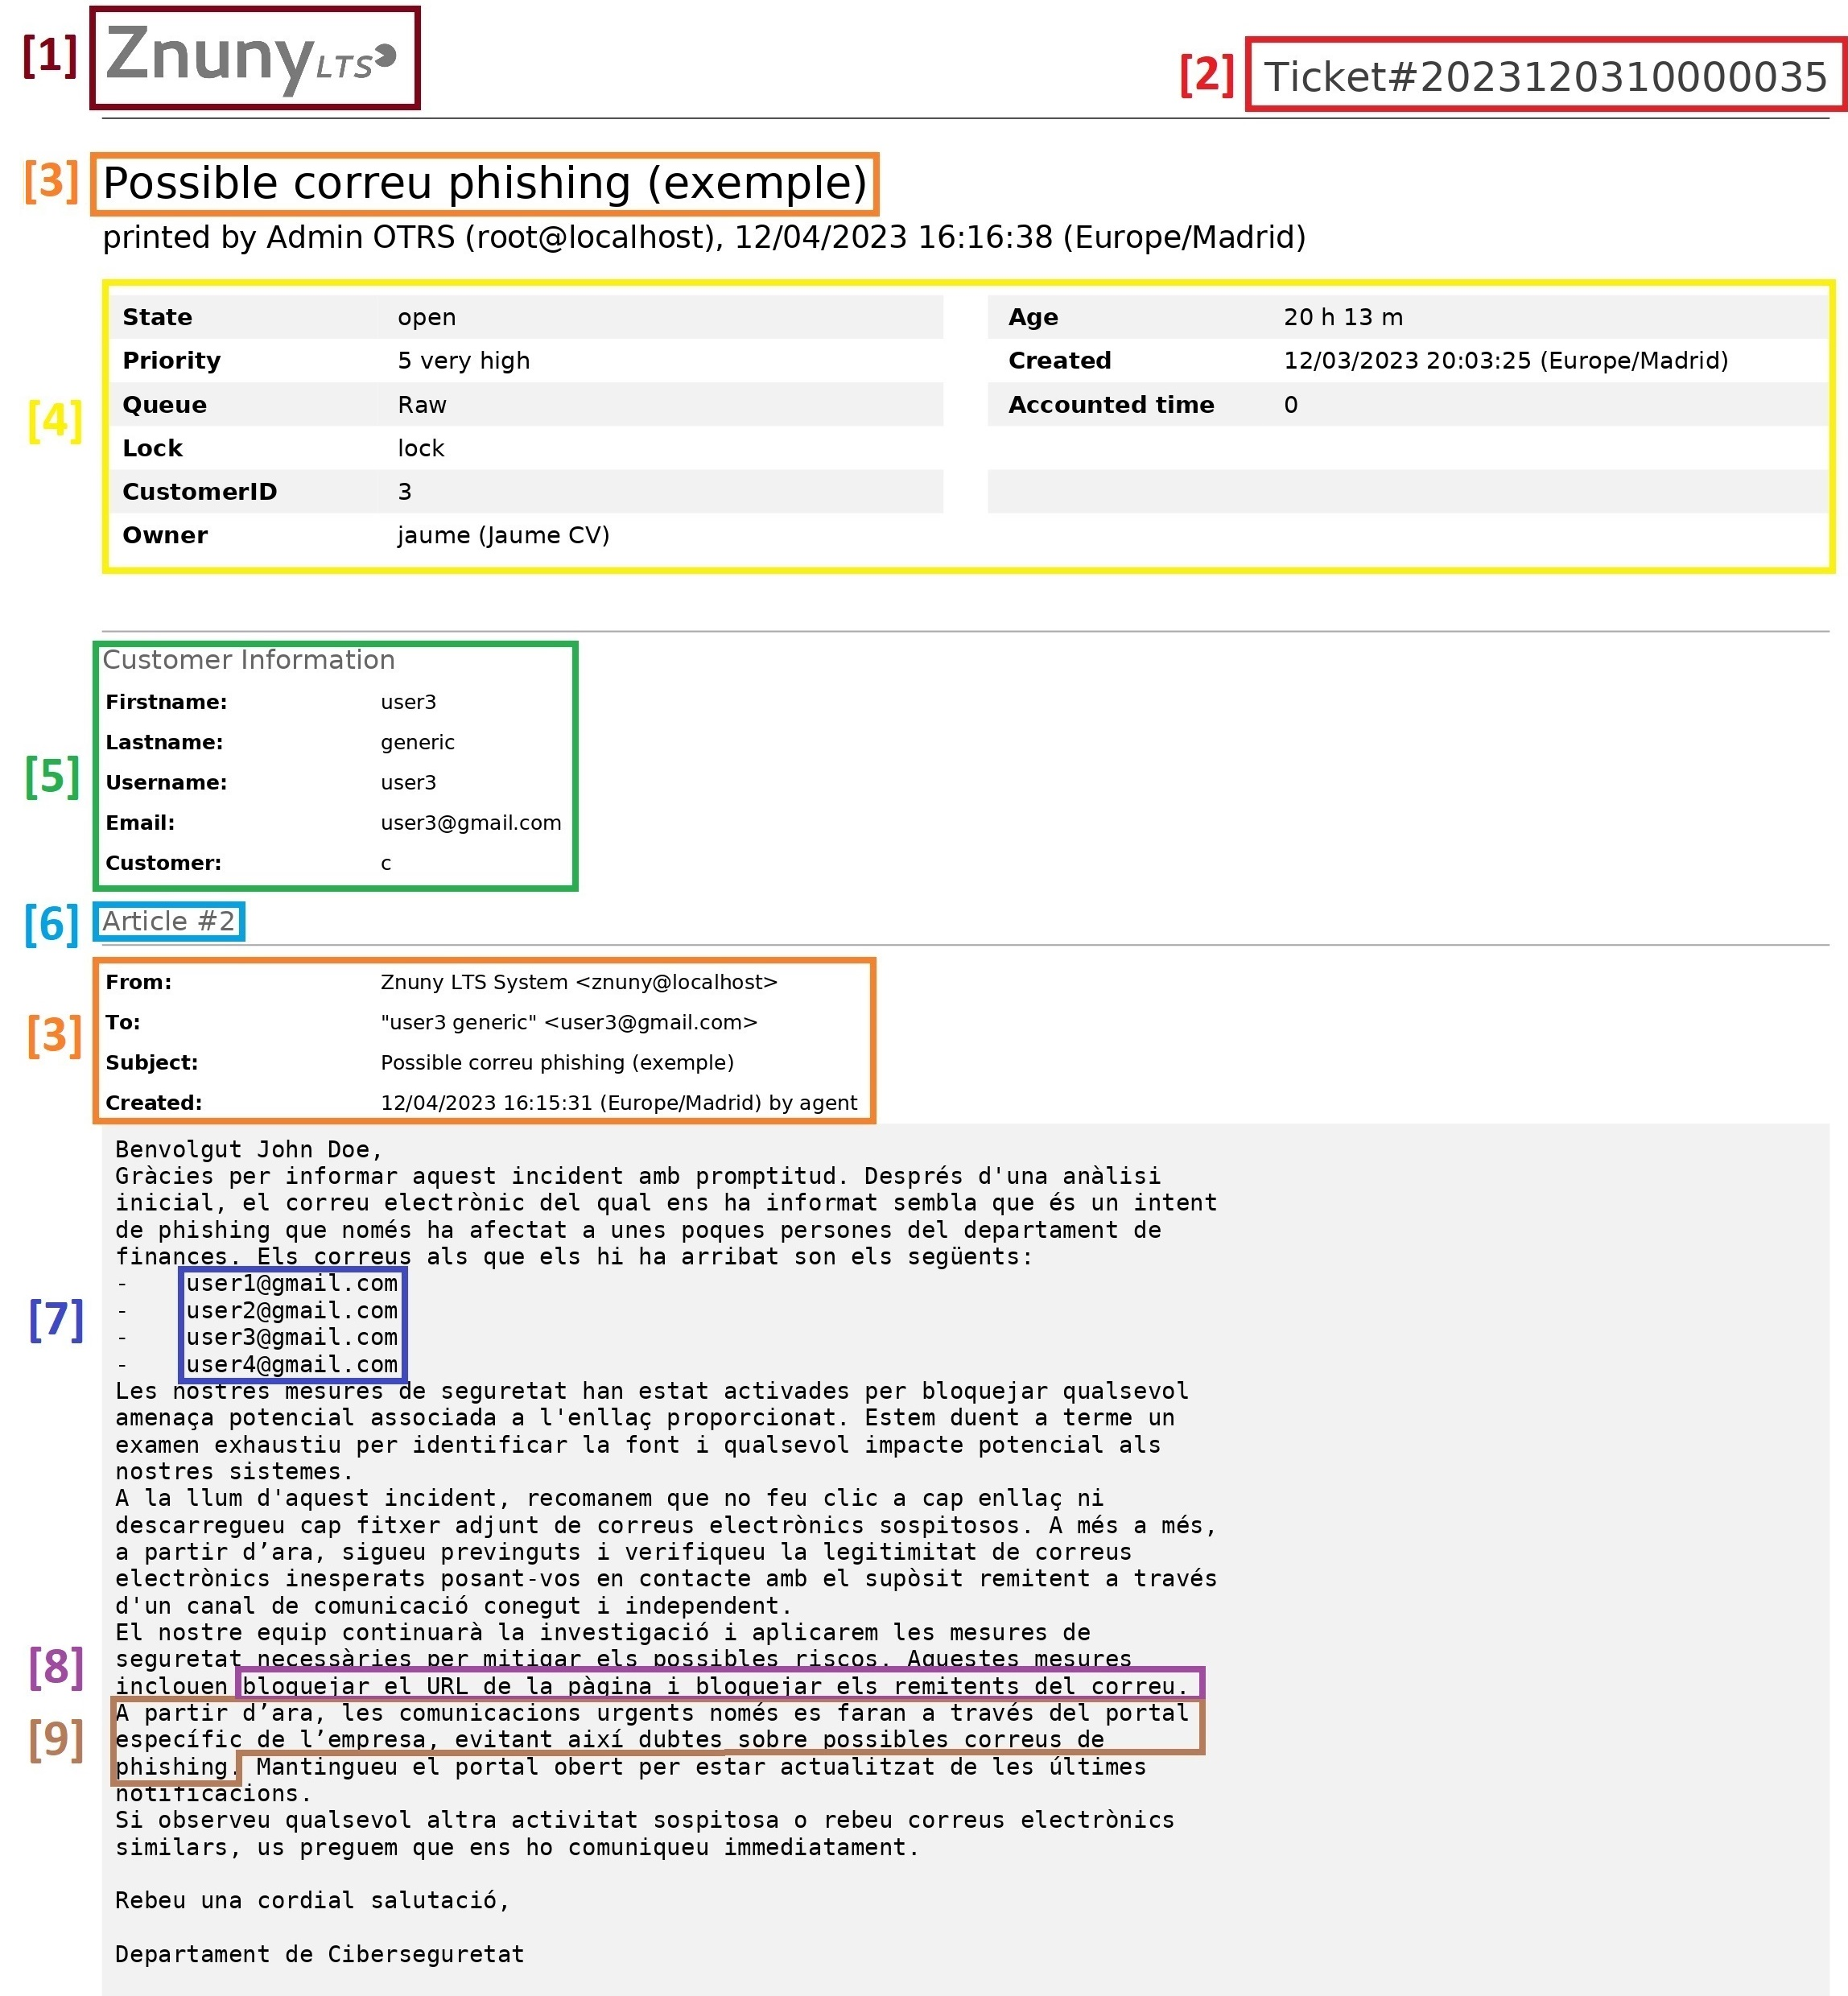
\includegraphics[width=\textwidth]{meitat-1.png}
    \caption[Primera meitat del tiquet d'exemple d'ORTS]{Primera meitat del tiquet d'exemple d'ORTS amb totes les parts indicades. \\ (Creació pròpia)}
    \label{fig:tiquet-exemple-1}
\end{figure}

\begin{figure}[H]
    \centering
    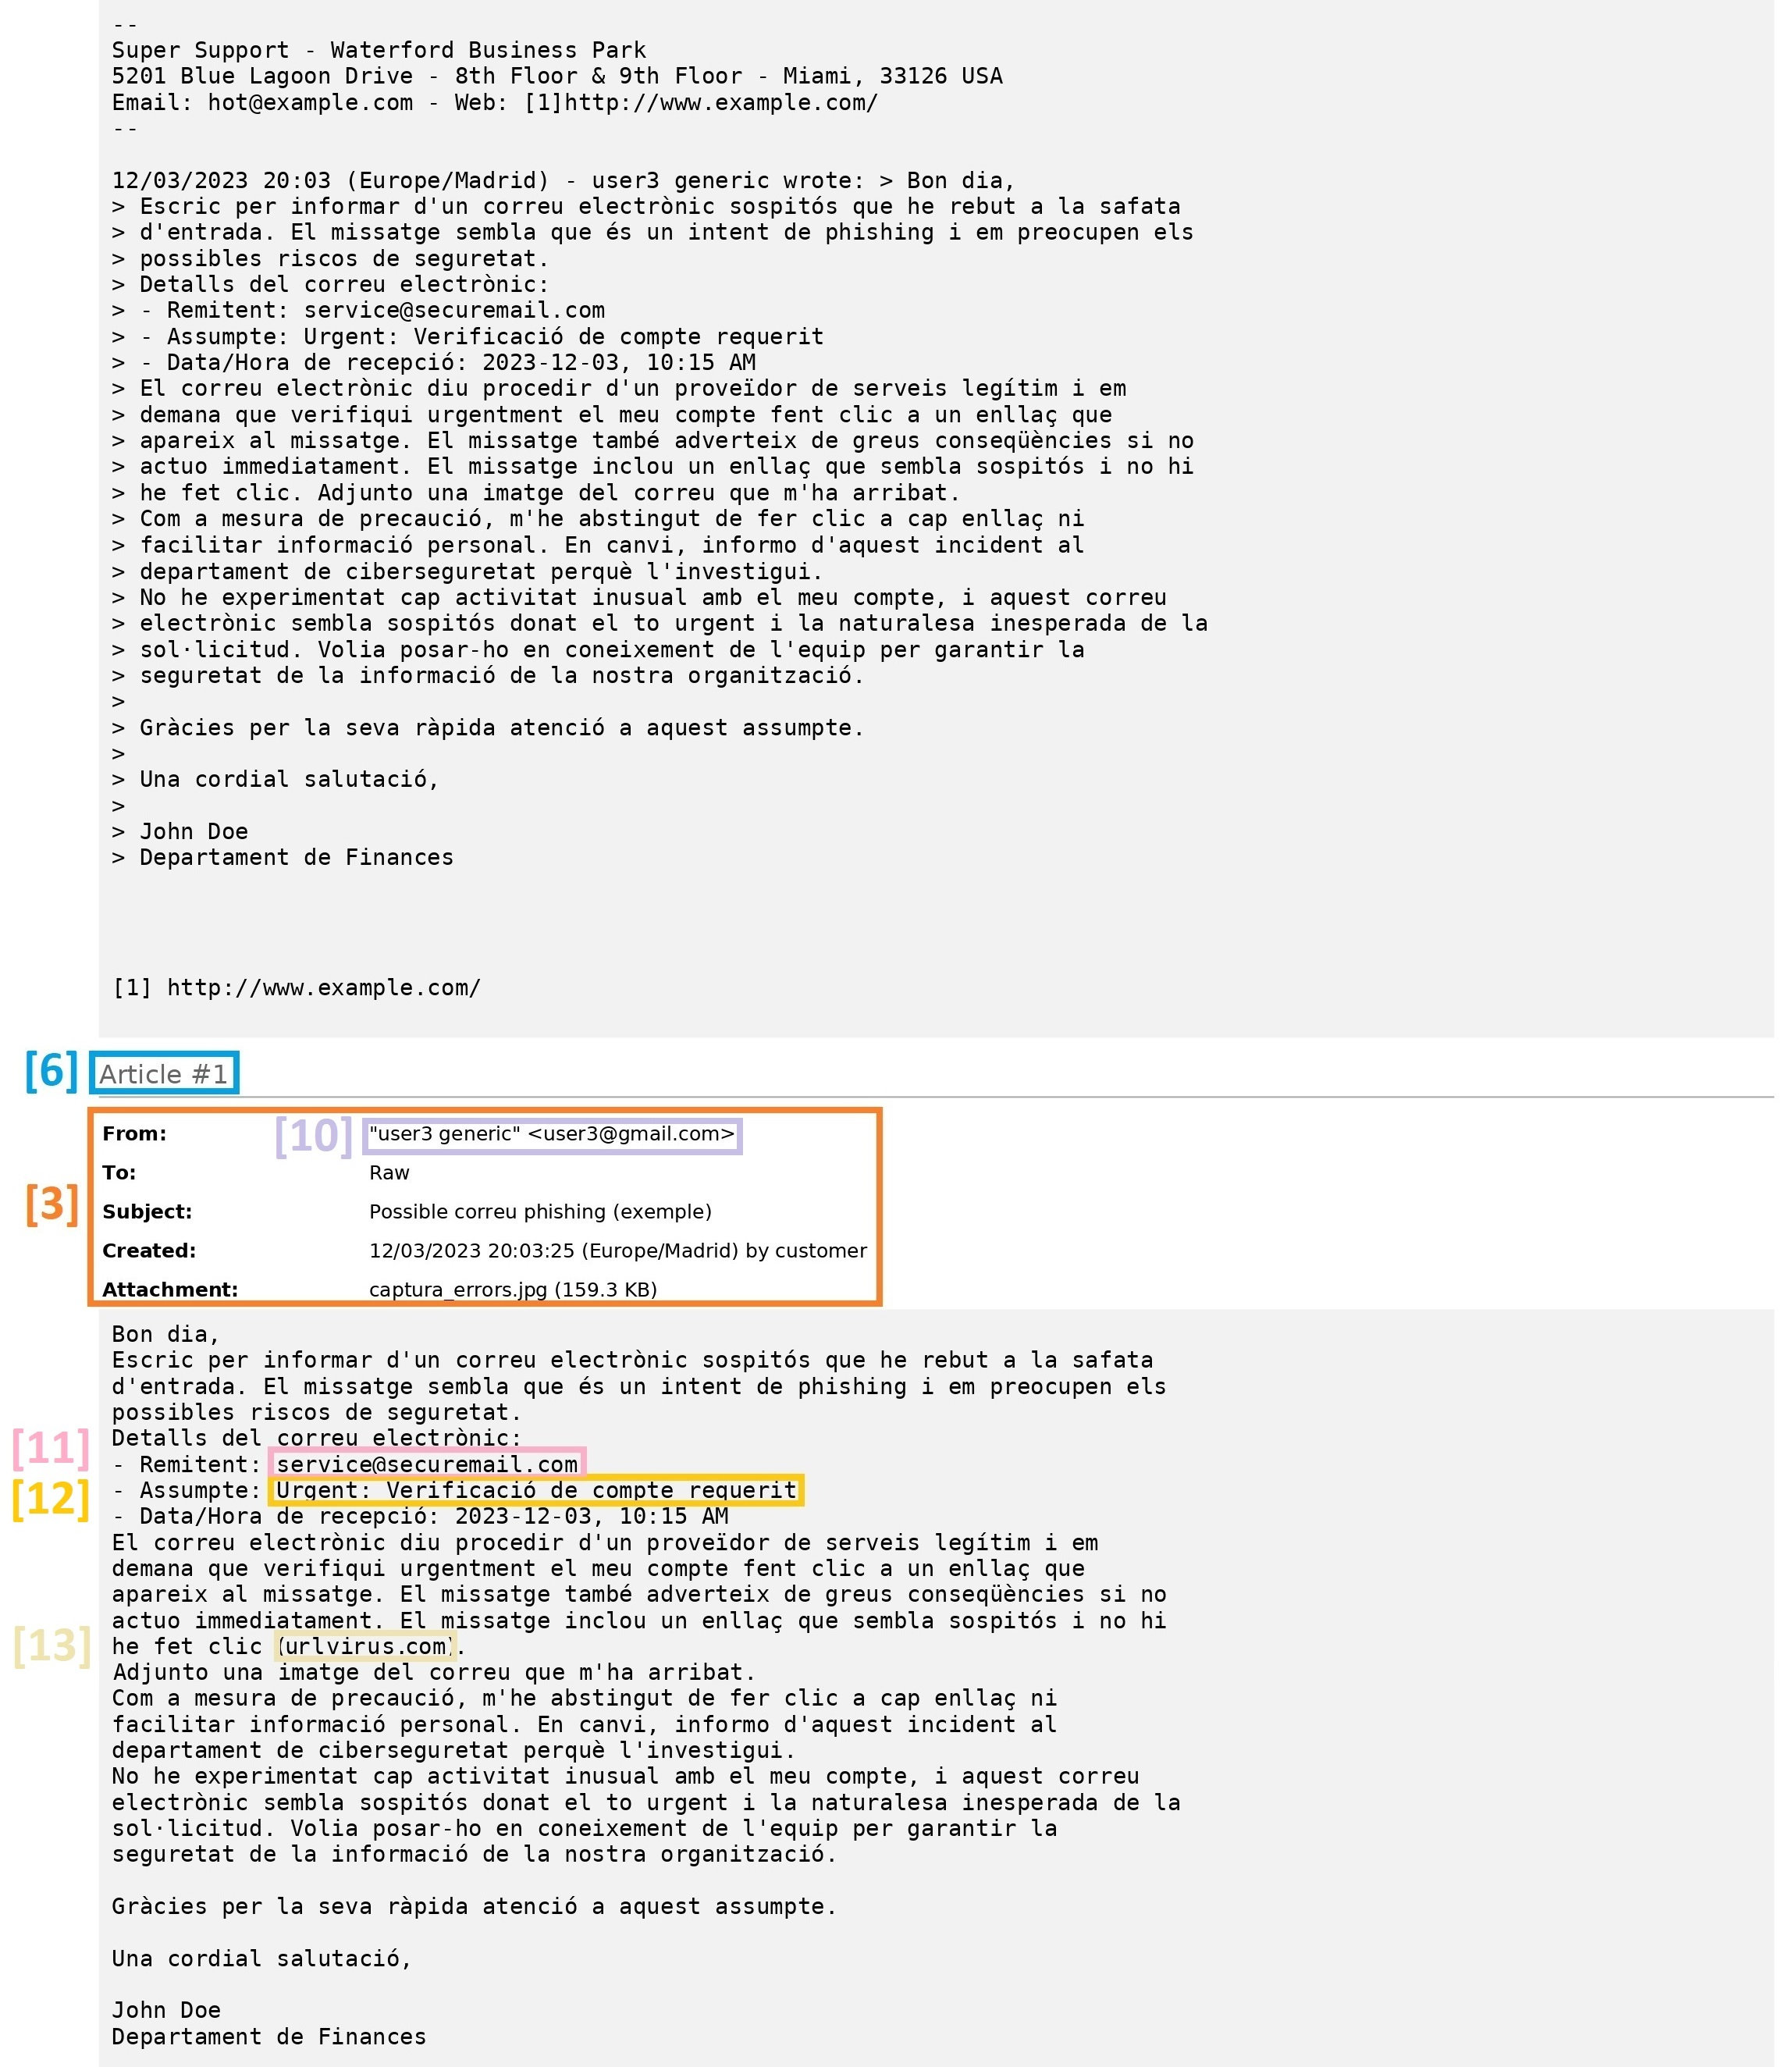
\includegraphics[width=\textwidth]{meitat-2.png}
    \caption[Segona meitat del tiquet d'exemple d'ORTS]{Segona meitat del tiquet d'exemple d'ORTS amb totes les parts indicades. \\ (Creació pròpia)}
    \label{fig:tiquet-exemple-2}
\end{figure}


\subsubsection{Non-Disclosure Agreement (NDA)}
Un acord de no divulgació (NDA), també conegut com a acord de confidencialitat, és un contracte legal que estableix una relació confidencial entre dues o més parts que acorden protegir qualsevol informació confidencial que puguin compartir o rebre.

Els elements clau d'un acord de confidencialitat solen incloure la identificació de la informació confidencial, la descripció de les obligacions i les responsabilitats de les parts reveladora i receptora, l'especificació de la durada i l'abast de les obligacions de confidencialitat, i la definició de les excepcions o exclusions de l'acord. En cas d'incompliment d'un acord de confidencialitat per una de les parts, l'altra part o les altres parts poden sol·licitar recursos legals, com ara mesures cautelars o danys i perjudicis, per evitar noves divulgacions i compensar qualsevol pèrdua.

En aquest context, l'acord de confidencialitat que s'ha signat per aquest projecte, inclou la protecció de totes les dades que estiguin dins dels servidors de l'\textbf{Agència} (en especial els tiquets d'incidències), així com tota l'informació relativa al projecte que contingui informació crítica. Això implica no poder usar cap servei que impliqui moure les dades fora dels servidors.

\subsubsection{Phishing}
El \textit{phishing} és un tipus de ciberatac que utilitza correus electrònics fraudulents o altres mètodes de comunicació per enganyar els destinataris per tal que revelin informació confidencial o instal·lin \textit{malware} als seus dispositius. Sovint, els correus electrònics de \textit{phishing} suplanten la identitat d'entitats o persones legítimes i redirigeixen els usuaris a pàgines web falses dissenyades per assemblar-se als reals. El \textit{phishing} pot donar lloc a robatoris d'identitat, pèrdues financeres o comptes compromesos.

\subsubsection{Malware}
El \textit{malware} o programari maliciós es refereix a qualsevol programa dissenyat per interrompre o danyar un sistema informàtic, una xarxa o un dispositiu. El \textit{malware} pot dur a terme una sèrie d'accions malicioses, entre les quals s'inclouen robar, xifrar o esborrar dades i monitorar l'activitat de l'usuari. També es pot infiltrar en els sistemes a través de diversos canals, com ara correus electrònics de \textit{phishing}, descàrregues de fonts no segures, mitjans extraïbles o connexions de xarxa. Un cop dins, el \textit{malware} pot suposar greus amenaces per a la seguretat del sistema, i, fins i tot, pot permetre ciberatacs addicionals.

\subsubsection{Dataset}
Un \textit{dataset} o conjunt de dades són les dades utilitzades per entrenar, validar i provar els models d'aprenentatge automàtic. És un element essencial de l'aprenentatge automàtic, ja que proporciona les dades necessàries perquè el model adquireixi coneixements i generi prediccions. Depenent del problema que s'abordi, pot incloure dades en diferents formats, com ara text, imatges o àudio. La informació d'un \textit{dataset} sol tenir etiquetes, cosa que indica que cada entrada sol tenir una sortida esperada. Aquestes etiquetes són útils per entrenar el model a distingir patrons a la informació rebuda i generar prediccions precises per a dades mai vistes abans. Per crear un \textit{dataset} de la màxima qualitat cal considerar meticulosament el procés de recopilació, neteja i etiquetatge. És crucial garantir que el conjunt de dades representi amb precisió el problema que s'aborda i contingui prou informació per entrenar eficaçment el model.
